\documentclass[12pt]{article}
%Gummi|065|=)
\usepackage{amsmath, amsfonts, amssymb}
\usepackage[margin=0.5in]{geometry}
\usepackage{xcolor}
\usepackage{graphicx}

\newcommand{\off}[1]{}
\DeclareMathSizes{20}{30}{20}{18}

\newcommand{\two }{\sqrt[3]{2}}
\newcommand{\four}{\sqrt[3]{4}}


\usepackage{tikz}

\title{Nilsequences}
\author{John D Mangual}
\date{}
\begin{document}

\fontfamily{qag}\selectfont \fontsize{12.5}{15}\selectfont

\maketitle

\noindent Terence Tao sees a lot of things, but he writes in an obfuscated way, and I think he misses a lot of things.  About 10 years ago, I was introduced to the topic of \textbf{nilsequences} in a course of Dynamics and Number Theory.  I did nothing with it.  Let's read Terry's latest blog on this topic\footnote{\texttt{https://terrytao.wordpress.com/2017/04/28/notes-on-nilcharacters-and-their-symbols/}}. \\ \\
Part of it is like\dots where do fractions come from?  \\ \\
If we take scientific measurement, there's quite a bit error that obstructs us from observing the most delicate patterns.  In fact, shielding us completely from finding them (or protecting us). \\ \\
$\sqrt{2} = 1.414213562373095048801688724209698078
5696718753769480731766797379907324784621070388503 $ \\ \\
If you examine the digits carefully\footnote{\texttt{http://www.gutenberg.org/files/129/129.txt}} we can prove the decimals do not exhibit any pattern in the decimal expension.  However, if we use continued fractions: \\ \\
$\sqrt{2} = [1; 2,2,2,2,2 , \dots ] $
and this is a nicer system since we have exponential convergence of the the number.  Here the error is $10^{-6}$ (microscopic). \\ \\
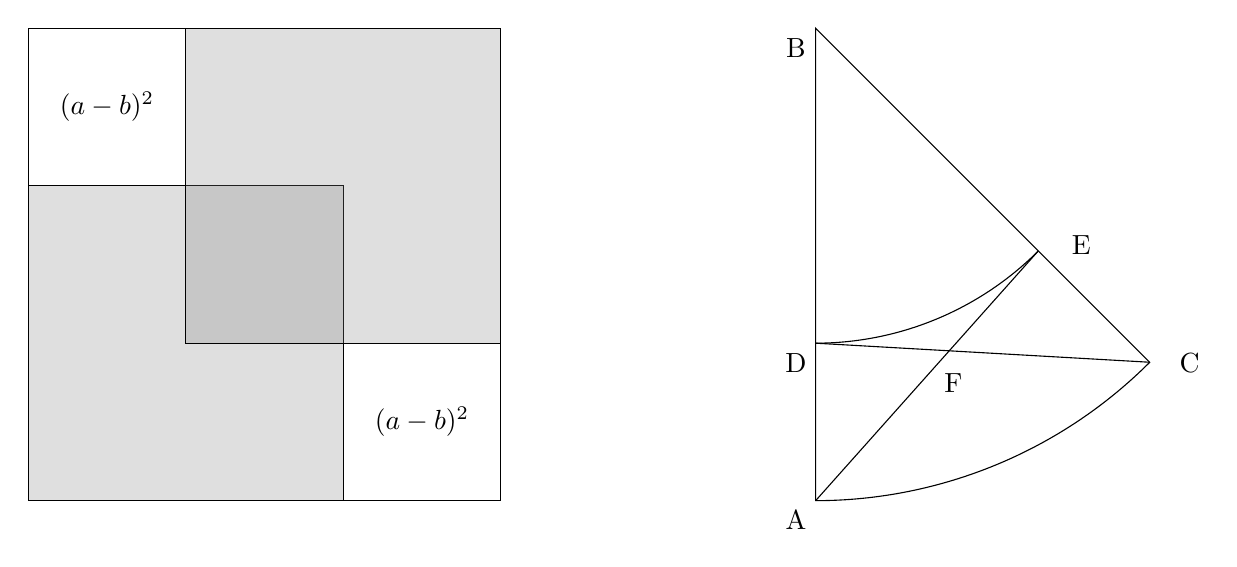
\begin{tikzpicture}

\begin{scope}
\draw (0,0)--(6,0)--(6,6)--(0,6)--cycle;
\draw[opacity=0.25, fill=black!50!white] (0,0)--(4,0)--(4,4)--(0,4)--cycle;
\draw (0,0)--(4,0)--(4,4)--(0,4)--cycle;
\draw[opacity=0.25, fill=black!50!white] (2,2)--(6,2)--(6,6)--(2,6)--cycle;
\draw (2,2)--(6,2)--(6,6)--(2,6)--cycle;
\node at (1,5) {$(a-b)^2$};
\node at (5,1) {$(a-b)^2$};
\end{scope}

\begin{scope}[xshift=10cm]

\draw (0,6)--(0,0)--(0,0) arc (90:135:-6)--cycle;
\draw (0,2) arc (90:135:-4);
\node at (-0.25,-0.25) {A};
\node at (-0.25,-0.25+6) {B};
\node at (-0.25+5,-0.25+2) {C};
\node at (-0.25,-0.25+2) {D};
\node at (-0.25+3.625,-0.25+3.5) {E};
\node at (-0.25+2,-0.25+1.75) {F};
\draw (0,2)--(6*1.414/2, 6 - 6*1.414/2);
\draw (0,0)--(4*1.414/2, 6 - 4*1.414/2);

\end{scope}

\end{tikzpicture} \\
These pictures lead to two different proofs that $\sqrt{2} \notin \mathbb{Q}$.  They are both geometric proofs, and argue by infinite descent.  Therefore, there must have been an \`{e}tale cohomology. \\ \\
I have no idea what \`{e}tale cohomology and the books do not simplify it enough for me. \\ 
Forget it.  One way to get meaningful numbers to arbitrary accuracy is to observe a dynamical system over time and take detailed measurements.  And you will see.

\newpage

\noindent Using a minimimal amount of math we can define most (possibly all) nilsequences.  The fractional part of multiples of $\sqrt{2}$ is nilsequence. \\

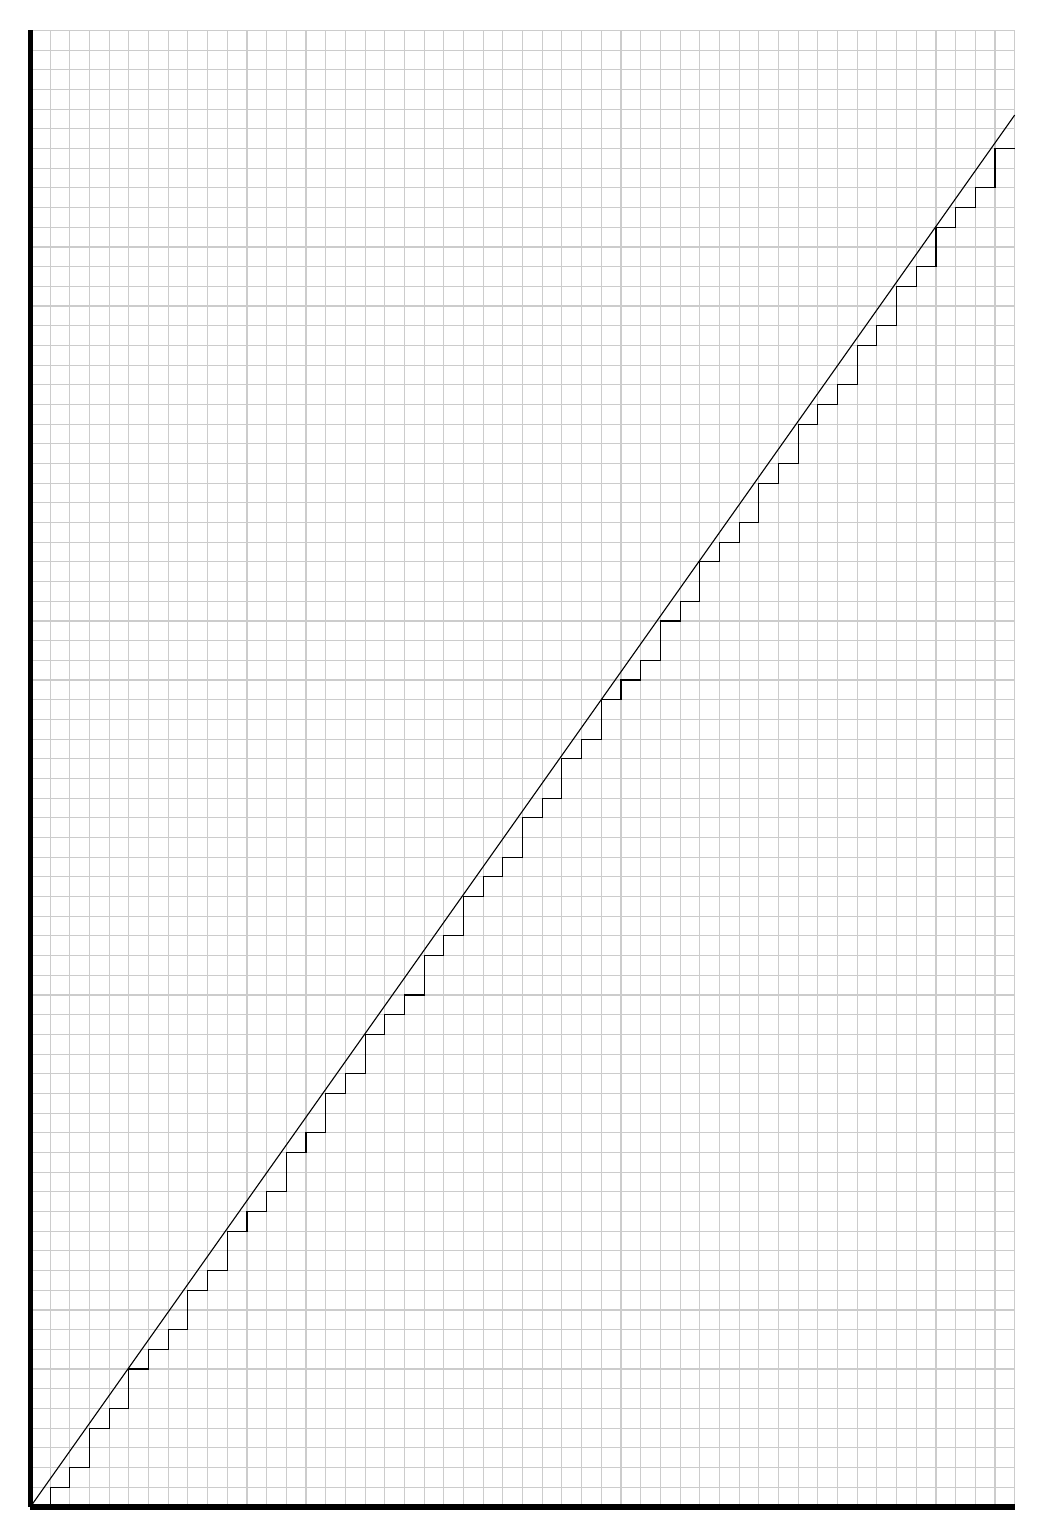
\begin{tikzpicture}[scale=0.25]

\foreach \a in {0,...,50}{
	\draw[color=black!20!white] (\a, 0)--(\a, 75);
}

\foreach \a in {0,...,75}{
	\draw[color=black!20!white] ( 0,\a)--( 50,\a);
}

\draw (0,0)--(1,0)-- (1,1)--(2,1)-- (2,2)--(3,2)-- (3,4)--(4,4)-- (4,5)--(5,5)-- (5,7)--(6,7)-- (6,8)--(7,8)-- (7,9)--(8,9)-- (8,11)--(9,11)-- (9,12)--(10,12)-- (10,14)--(11,14)-- (11,15)--(12,15)-- (12,16)--(13,16)-- (13,18)--(14,18)-- (14,19)--(15,19)-- (15,21)--(16,21)-- (16,22)--(17,22)-- (17,24)--(18,24)-- (18,25)--(19,25)-- (19,26)--(20,26)-- (20,28)--(21,28)-- (21,29)--(22,29)-- (22,31)--(23,31)-- (23,32)--(24,32)-- (24,33)--(25,33)-- (25,35)--(26,35)-- (26,36)--(27,36)-- (27,38)--(28,38)-- (28,39)--(29,39)-- (29,41)--(30,41)-- (30,42)--(31,42)-- (31,43)--(32,43)-- (32,45)--(33,45)-- (33,46)--(34,46)-- (34,48)--(35,48)-- (35,49)--(36,49)-- (36,50)--(37,50)-- (37,52)--(38,52)-- (38,53)--(39,53)-- (39,55)--(40,55)-- (40,56)--(41,56)-- (41,57)--(42,57)-- (42,59)--(43,59)-- (43,60)--(44,60)-- (44,62)--(45,62)-- (45,63)--(46,63)-- (46,65)--(47,65)-- (47,66)--(48,66)-- (48,67)--(49,67)-- (49,69)--(50,69);

\draw (0,0)--(50,1.414*50);

\draw[line width = 2] (0,0)--(50,0);
\draw[line width = 2] (0,0)--(0,75);

\end{tikzpicture} \\ 
We want\dots even more nilsequences.  In the Terry Tao blog we get two to get us started:
$$ n \mapsto \big( \sqrt{2} n  \{ \sqrt{3} n \} \big) \text{ or } n \mapsto \big( \sqrt{2} n  \{ \sqrt{2} n \} \big) $$
Earlier, two professors Vitaly Bergelson and Alexander Leibman studied these kinds of sequences of numbers, to my satisfaction. \\ \\
Green and Tao are looking for patterns in sequences of numbers.  I can never produce a sequence of numbers that would require the techniques they are using.  And yet, we kind of see them every day.

\newpage

\noindent In empirical measurements; any time we try to use math to solve a real problem, things get ``complicated" and maybe Green and Tao help us reason about that. \\ \\
Tao's blog today was about \textbf{symbols} of nilsequences.  I don't understand how you can write an entire theory of numbers and still not write down a single one.  We can compute:
$$ n \times  \left( \begin{array}{ccc} 
1 & x & y \\ 0 & 1 & z \\ 0 & 0 & 1 \end{array} \right)
 = \left( \begin{array}{ccl} 
1 & n \, x & n\, y + \binom{n}{2} \, x z\\ 0 & 1 & n \, z \\ 0 & 0 & 1 \end{array} \right) $$
The notation $n \times \cdot \equiv (\,\cdot \,)^n$ is short for multiplying a number by itself $n$ times.  Here $x$, $y$, $z$ are elements of $\mathbb{R}$, but they could also be elements of $\mathbb{Z}$.  And it's the number in the upper right corner we are intested.  So, if you do the reduction right you get 
$$ n \mapsto ( \{ n x \} , \{ ny + nx \lfloor nz \rfloor \} , \{ n z\} ) $$
and I'm faking it slightly because I haven't done the arithmetic.  \\ \\
It helps to think like a cave man.  What if there were no numbers?  We could take two lengths and add them. \\ \\
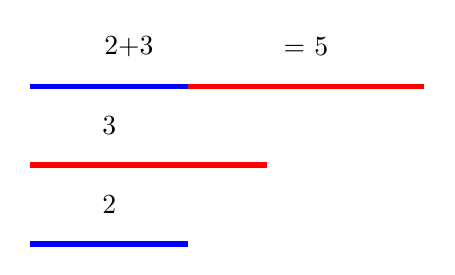
\begin{tikzpicture}

\draw[blue, line width=2 ] (0,2)--(2,2);
\draw[red , line width=2 ] (2,2)--(5,2);
\draw[red , line width=2 ] (0,1)--(3,1);
\draw[blue, line width=2 ] (0,0)--(2,0);

\node at (1,0.5) {2};
\node at (1,1.5) {3};
\node at (1.25 ,2.5) {2+3};
\node at (3.5,2.5) {= 5};

\end{tikzpicture} \\ \\
Tao - and Green, somewhat - have become suspect of the basic number operations.  $+$, $\times$, $-$, $\div$ if you do it too much and then someone tells you that it's wrong. So, let's try  new kind of number!

\newpage

\noindent \textbf{5/2} I would like to try to fill in the part about Galois cohomology.  Leading to the side issues like dynamics and computabiity, so the scenery is very rich.  \\ \\
We are trying to show that $x^2 = 2$ has no solutions in rational number $x \in \mathbb{Q}$ or (clearing denominators) $a^2 = 2b^2 $ has no solutions $a,b \in \mathbb{Z}$.  There seems to be a way using \textbf{heights} and a way using \textbf{torsors} but every book reviews it differently.  And hopefully we see what this cohomology nonsense is about. \\ \\
\textbf{\#1} The ``height" of a fraction $\frac{a}{b}$ is just the numerator plus the denominator $|a| + |b|$.
$$  h \big(\frac{2}{3}\big) = |2| + |3| = 5$$
what is the hehgit of a fraction that could represent the $\sqrt{2}$ ?  We could have that:
$$ h(2) = h(\tfrac{2}{1}) = 2 = h(\tfrac{a^2}{b^2})  = a^2 + b^2$$
here I used the symbol ``=" to mean the English word ``but also" and $(a,b) = 1$ the numbers $a$ and $b$ are \textbf{relatively prime}.  How can two integers, have a square that sums to two?  
$$ a^2 + b^2 = 1 \longrightarrow a = b = 1 $$
That's not possible.   \\ \\
The find print is, we could find completions where $\sqrt{2}$ exists, such as $\mathbb{R}$ or $\mathbb{Q}_3$ or any $\mathbb{Q}_p$ when $\frac{p^2-1}{8}\in \mathbb{Z}$ is an even number\footnote{\texttt{https://mixedmath.wordpress.com/2012/08/23/an-elementary-proof-of-when-2-is-a-quadratic-residue/}}. \\ \\
\textbf{\#2} These math textbooks give really deep names to really basic concepts.  Continuing with $\sqrt{2}$
$$ x^2 - 2y^2 = (x - \sqrt{2} y) ( x + \sqrt{2}y )=  1 $$
One way to phrase this is that we have adjoint $\sqrt{2}$ to the ring of integers $\mathbb{Z}$ and obtained $\mathbb{Z}[\sqrt{2}]$.  Bjorn Poonen defines an affine variety (an ``equation"):
$$ x^2 - 2y^2 = -3  \text{ over } \mathbb{A}_\mathbb{Q}$$
In his notation $\mathbb{A}_\mathbb{Q} = \mathrm{Spec}\; \mathbb{Q} $ is the ``line" while $\mathbf{A}_\mathbb{Q}$ are the Adeles.  I think $\mathrm{Spec}\;\mathbb{Q}$ is just $\mathbb{Q}$. So we are trying to solve this equation over fractions.  We don't know if there are any solutions just yet. \\ \\
He defines a \textbf{torus} -- a term which throws me completely off because it is a hyperbola.
\begin{itemize}
\item $T = \{ x^2 -2y^2 = 1 \} \subseteq \mathbb{A}_\mathbb{Q}^2 = \mathrm{Spec} \; \mathbb{Q}[x,y]$
\item there is some kind of multiplication: $\mathbf{\times}: T \times T \to T$
\item $(x_1,y_1) \times (x_2,y_2) = ( x_1 x_2 + 2 y_1 y_2 , x_1 y_2 + x_2 y_1)$
\end{itemize}
The real definition of torus is the most obnoxious thing ever: it is a twist on $\mathbb{G}_m^n$ (as a group scheme), where $\mathbb{G}_m = \mathrm{Spec}\; \mathbb{Q}[t, t^{-1}] $ and $m$ stands for ``multiplication".
\newpage

\noindent This guy really emphasizes schemes and he considers $\mathrm{Spec}[ \; \cdot \; ]$ a lot (this is a \textbf{functor})\\ \\We can look for different points on curves, and there will be a torus action:
$$ x^2 - 2y^2 = - 3 \quad\text{ or }\quad x^2 - 2y^2 = 0 $$
The last one might be a scheme and not a variety.\footnote{The book is written in such a formal way, it's hard to understand.  Can't say I'm doing a great job.}  In both cases, $X(\mathbb{Q}) = \varnothing$ (there are no rational ``points") in either case so\dots this is a non-trivial $T$-torsor. \\ \\
For any fixed smooth algebraic group $G$ (in our case, the solutions to $x^2 - 2y^2 = 1$ with multiplication and we will write it $T$) these three objects are thes same: 

\begin{itemize}
\item $T$-torsor over $\mathbb{Q}$
\item twists of $\mathbf{G}$ (possibly $\mathbf{G}$)
\item $H^1(\mathbb{Q}, T)$
\end{itemize}
if $X = \{ x^2 - 2y^2 = 0 \}$ is a torsor it has a cohomology the cohomology class. $$[\{ x^2 - 2y^2 = 0 \}] \in H^1 \big(\mathbb{Q}, \{ x^2 - 2y^2 = 1\} \big)$$ 
$\mathbf{G}$ is the \textbf{trivial torsor}  (Grothendieck thought math centered around the notion of zero, which took thousands of years to develop.  So we have all thse notations for zero-like concepts.). \\ \\
$\sqrt{2} \notin \mathbb{Q}$ how can our torsor have any points? \\ \\
We have to examine the \textbf{separable closure} $\mathbb{Q}_s$ -- I have never seen so many numbers in my life.  Hopefully if we adjoin enough numbers, $\sqrt{2}$ is in there.  Maybe
$$ \mathbb{Q}(\sqrt{2}) = \mathbb{Q}[x]/(x^2 - 2) $$
will be enough. \\ \\
I haven't really said what ``cohomology" is.  Any function $\mathbb{Q} \to T$ is an element of cohomology and the ``class" is just a way of declaring two of these two be the same.  These equivalences form a hierarchy. \\ \\
I am thinking the end result here is not a ``proof" but an exhibition of how all the machinery is connected. \\ \\ 
I guess ``torsor" was just another wod for ``equation".  The idea was there should be a local to global principle:
$$ H^1(\mathbb{Q}, G) \stackrel{1:1}{\longrightarrow} \prod_{p \in \text{prime}} H^1(\mathbb{Q}_p, G) $$
the real idea is that if you want to solve the equation in $\mathbb{Q}$ you should try to solve the equation in $\mathbb{Q}_p$ for all prime numbers $p$ (and also $\mathbb{R}$). A cohohomology class $[X] \in H^1(\mathbb{Q}, G)$ is just an equation and $[X]=0$ means we can solve it.
\\ \\
\noindent Having exceeded the time cap for this approach, we pick a new one.\footnote{We'll review it more later.  There is Neukirch's \textbf{Cohomology of Number Fields} (which is like the sequel to his textbook ``Algebraic Number Theory" and Jean-Pierre Serre \textbf{Galois Cohomology} and the question is always the same: how can we get these frameworks or theories to work for us? }.

\newpage 

\noindent \textbf{5/4} Christophe Soul\'{e} had me sold on this book for two reasons:  he promises a theory of infinite descent using \textbf{Arakelov geometry}.  As usual, not a single equation in sight. \\ \\
What blew me away was how, in passing, he writes down almost every thought on renormalization I've had; again only in the most general terms, leaving ``exercises" to the reader. \\ \\
He does write \textbf{(A)} $\infty ! = \sqrt{2\pi}$ and also \textbf{(B)} $\infty! = e^{-\zeta'(0)} $ leading to a kind of regularization:
$$ 1 \times 2 \times 3 \times 4 \times \dots = \sqrt{2\pi} $$
and the discussion quickly gets rather pretentious.  Yet, for the time being, we see that he is right. \\ \\
There is an extensive literature of zeta-functions.  There's a zeta function for Schemes.  Bjorn Poonen gives us:
$$ \zeta(s) = \sum_{n \geq 1} n^{-s} = \prod_{p = \text{prime}} \frac{1}{1-p^{-s}} = 
\prod_{\mathfrak{m}\in \text{maximal}} \frac{1}{1- \# (\mathbb{Z}/\mathfrak{m})^{-s}} = \prod_{P \in \mathrm{Spec}\mathbb{Z}} \frac{1}{1-\# \mathbb{Q}(P)^{-s}}$$
So $\mathbb{Z}$ is now the scheme $X = \mathrm{Spec} \mathbb{Z}$. In that section of the book he uses \'{e}tale cohomology\footnote{to prove the Hasse principle (local-global principle) we were using Galois cohomology.  It's tough to keep these straight.} The formulas that Soul\'{e} outlines for us a zeta function for any scheme $X$. \\ \\
It seems to be on me, what I want for an ``explicit computation".  Seems to be kind of a game.  We have an endless supply of zeta functions.  Let's write down one or two:
$$ \zeta(s)^2 = \left( \sum_{n \geq 1} n^{-s} \right)^2 = \sum_{n \geq 1} d(n) \, n^{-s} \neq \sum_{n \geq 1} r_2(n) \, n^{-s}  $$
here $r_2(n)$ is the number of way of writing $n$ as the sum of two squares.  $d(n)$ is \# of divisors.
$$ 50 = 5 \times 5 + 5 \times 5 = 7 \times 7 + 1 \times 1 = 1 \times 1 + 7 \times 7 $$
considerations like these lead to a very rich theory of modular forms; and there is all kinds of stuff.  I am wrong.  Sum of two squares is it's own zeta function.  I think it's 
$$ \zeta_{\text{Spec}\mathbb{Z}[i]}(s) = \left( \sum_{a,b} (a^2+ b^2)^{-s} \right)  = \sum_{n \geq 1} r_2(n) \, n^{-s} = \prod_{p = 4k+1} \dots \times \prod_{p = 4k+3} \dots $$
\textbf{Exercise} (i.e. I have no idea right now) find an appropriate Dirichlet series for the sum of two squares. \\ \\
\textbf{Discussion} Already did it.  There are two kinds of primes in $\mathbb{Z}[i]$, $p = 4k+1$ which split into $p = a^2 + b^2 = (a+bi)(a-bi) $ and $p = 4k+1$ which do not split.  This factorization result is not free, it uses a {\color{red!60!white}geometry of numbers} leads into {\color{blue}class field theory}.  
$$ \left( \sum_{a,b,c,d} (a^2+ b^2 + c^2 + d^2)^{-s} \right) =  \sum_{n \geq 1} r_4(n) \; n^{-s}  $$
There are lots of interesting zeta-functions and a rich complicated literature. I think it's our choice to pick an encoding back into ``elementary" number theory (if possible)

\newpage

\noindent Soul\'{e} has three approaches for understanding $\infty! = \sqrt{2\pi}$. \\ \\
\textbf{\#1} Stirling's formula let's us estimate the number of rearrangements of things:
$$  n! = 1 \times 2 \times 3 \times \dots \times \times  n = (n/e)^n \sqrt{2\pi n}$$
This formula can arise in two ways: gambling and estimation.
\begin{itemize}
\item $\binom{n}{k}$ the probability of flipping $n$ coints and getting $k$ heads and $n-k$ tails
\item $f(x + \epsilon) = \sum f^{(n)}(x) \frac{\epsilon^n}{n!}$ this is called \textbf{Taylor Series}; it's just the best fit line. we do it mentally
\end{itemize}
this is a low-fat way of getting all sorts of dualities.  Not rarefied enough for certain crowd but will have to suffice. Eventually I will return to the Terry Tao blog -- he has all kinds of yummy low-fat tricks for us to learn even if he writes in a somewhat obfuscated way that I don't like. \\ \\
Taking the logarithm of the Stirling series we get an informative identity:
$$ \log (n!) = \log 1 + \log 2 + \dots + \log n = n \log n - n + \log \sqrt{2\pi} + O(n^{-1})$$
We should already be suspicious of Soul\'{e}'s approach.  One of the inputs to his discussion is a derivaton Stirling formula: 
\begin{itemize}
\item where did that $\sqrt{2\pi}$ come from? 
\item our estimate works within $O(n^{-1})$ precision.  How good is that really?
\end{itemize}
\textbf{\#2} Another way is using ``the functional equation" of the zeta function.\footnote{Later, we will find a whole class of L-series which satisfy a function equation.  These sequences of are not the easiest to calculate.  Again, I think the hard part is linking these modular forms to the sequences of numbers we care about.}  As eveyone knows:
$$ \pi^{s/2} \Gamma(s/2) \zeta(s) = \pi^{(1-s)/2} \Gamma((1-s)/2)\zeta(1-s) $$ 
so far so good.  There is symmetry around $\mathrm{Re}(s) = \frac{1}{2}$.  And take derivaive of zeta function:
$$ - \, \zeta'(s) =  \sum_{n \geq 1} \log n \; n^{-s} = \Bigg|_{s = 0} \;\; \sum_{n \geq 1} \log n $$
So\dots why is $\sqrt{2\pi}$ a reasonable number here?  There is an estimate around $s=1$ (again not for free)
$$ \zeta(s) = \frac{1}{s-1} + \gamma + O(s-1) $$
This is a way of expressing that $\zeta(1) = \infty$ with a little information about what happens nearby.
$$ \zeta(1) = 1 + \frac{1}{2} + \frac{1}{3} + \frac{1}{4} + \dots = 1 
+ \left( \frac{1}{2} + \frac{1}{3} \right)
+  \left( \frac{1}{4} + \frac{1}{5} + \frac{1}{6} + \frac{1}{7} +\right) + \dots 
\geq 1 + 1 + 1 + \dots $$
Regularization is kind of a disaster.  The complex plane $\mathbb{C}$ is comparatively well-behaved compared to the infinite dimensional object actually being studied. \\ \\
There's also a switch between $\zeta(0)$ and $\zeta(1)$ which is OK because of this mirror. 

\newpage

\noindent Using facts from a good complex analysis textbook.  He shows that:\\
\begin{tikzpicture}
\node at (0,0) {$\displaystyle\Gamma(s+1)= \sqrt{\pi} 2^s \Gamma(\frac{s+1}{2})\Gamma(s + \frac{1}{2})$};
\node at (4, 0) {$\displaystyle\to$};
\node at (8, 0) {$\displaystyle \frac{\Gamma'(1)}{\Gamma(1)} = \log 2 + \frac{1}{2} \frac{\Gamma'(\frac{1}{2})}{\Gamma(\frac{1}{2})} + \frac{1}{2}\frac{\Gamma'(1)}{\Gamma(1)}$};
\node at (11.5, 0) {$\displaystyle\to$};
\node at (14, 0) { $\displaystyle - \frac{1}{2} \frac{\Gamma'(\frac{1}{2})}{\Gamma(\frac{1}{2})} = 2 + \frac{\gamma}{2}$ };
\node at (14,1) {$\displaystyle\downarrow$};
\node at (14,2) {$\displaystyle \gamma = - \Gamma'(1)$};
\end{tikzpicture} \\ 
This is how I think of derivations: organized in two dimensions.   In the modern language these are expressed in terms of injective maps, exact sequences, modules and cohomology.  I hate it so much!  \\ \\
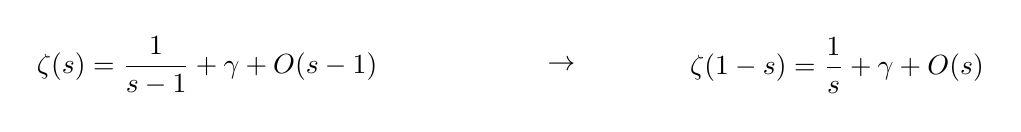
\begin{tikzpicture}
\node at (0,0) { $\displaystyle \zeta(s) = \frac{1}{s-1} + \gamma + O(s-1) $ };
\node at (4.5,0) {$\to$};
\node at (8,0) { $\displaystyle \zeta(1-s) = \frac{1}{s} + \gamma + O(s) $ };
\end{tikzpicture} \\ \\
This one is much clearer: subsitute $s \mapsto 1 - s$.  And we do these gymnastics, but now we organize into a careful way.  The only factorial identity we haven't used yet is the most basic one: \\ \\
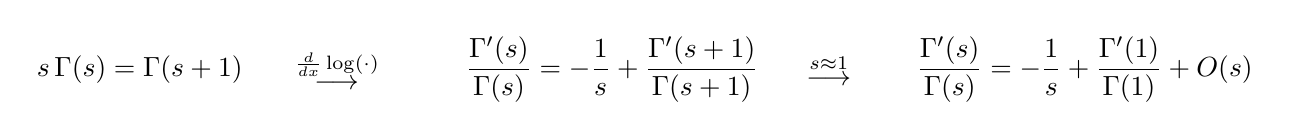
\begin{tikzpicture}
\node at (0,0) {$ s\, \Gamma(s) = \Gamma(s+1) $};
\node at (2.5,0) {$\stackrel{ \frac{d}{dx} \log (\cdot )}{\longrightarrow}$};
\node at (6,0) {$\displaystyle \frac{\Gamma'(s)}{\Gamma(s) } = - \frac{1}{s} + \frac{\Gamma'(s+1)}{\Gamma(s+1) } $} ;
\node at (8.75,0) {$\stackrel{s\approx1}{\longrightarrow}$};
\node at (12,0) {$\displaystyle \frac{\Gamma'(s)}{\Gamma(s) } = - \frac{1}{s} + \frac{\Gamma'(1)}{\Gamma(1) } + O(s)$};
\end{tikzpicture} \\
To me this makes more sense that the equations are being chain togeter this way.  Lastly:
$$ \frac{\zeta'(0)}{\zeta(0)} = \log 2 + \log \pi \text{ and } \zeta(0) = - \frac{1}{2} \text{ so that } \zeta'(0) = - \frac{1}{2} \log 2\pi  $$
This is my crude protoype for group cohomology: writing a bunch of equations in an organized way (using $\times$ and $+$). \\ \\
\textbf{\#3} (Divergent Integrals) \\ \\
The last template Soul\'{e} gives us has to do with theta functions and Mellin transforms: \\ \\
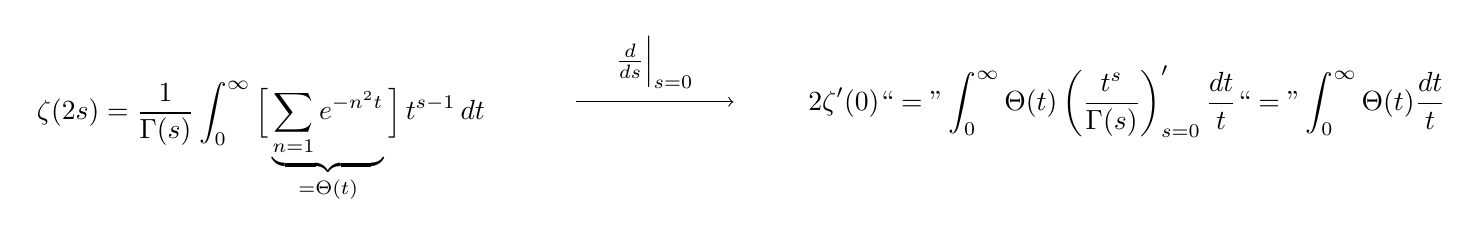
\begin{tikzpicture}
\node at (0,0) { $\displaystyle \zeta(2s) = \frac{1}{\Gamma(s)} \int_0^\infty \Big[ \underbrace{\sum_{n=1} e^{-n^2 t}}_{=\Theta(t)} \Big] \, t^{s-1} \, dt $ };
\draw[->] (4,0.5)--(6,0.5);
\node at (5,1) {$\frac{d}{ds}\Big|_{s=0}$};
\node at (11,0.5) {$\displaystyle 2 \zeta'(0) ``=" \int_0^\infty \Theta(t) \left( \frac{t^s}{\Gamma(s)} \right)'_{s=0} \frac{dt}{t} 
``=" \int_0^\infty \Theta(t)  \frac{dt}{t}$};
\end{tikzpicture} \\ 
Poisson summation is related to the map $t \mapsto - \frac{1}{t}$ in $SL(2, \mathbb{Z})$. 
$$ \Theta(t) = \sqrt{\tfrac{\pi}{t}} \Theta(\tfrac{\pi}{t})  - \frac{1}{2} 
 \quad\stackrel{t\approx 0}{=}\quad \tfrac{1}{2}\sqrt{\tfrac{\pi}{t}} - \tfrac{1}{2}   + O(\sqrt{t})$$
The [[derivative of the Mellin transform near $0$]] of $\Theta(t)$ is divergent and we can pick out the bad parts:
$$ \int_\epsilon^\infty \Theta(t)  \frac{dt}{t}
 = \# + a_0 \log \epsilon + \frac{a_{-1}}{\sqrt{\epsilon}} $$
 Regularization of infinite products involves doing stuff like this; just a bit old-fashioned yet lots of uncharted territory.\footnote{It's not hard to write an infinite product we'd be curious about (that is not just recycling the example we just did), and maybe it's important to a Math or Physics professor somewhere.}

\newpage

\noindent We still haven't shown $\sqrt{2} \notin \mathbb{Q}$ is irrational. \dots \\ \\
Just trying to get a sense of what this machinery is like and why it's there.  
\begin{itemize}
\item $X \subseteq \mathbb{P}^N$ is a bunch of equations
\item $\hat{X} \in \widehat{CH}(\mathbb{P}^{N-d}) $ is an ``arithmetic cycle" or whatever
\item $\hat{c}_1(\mathcal{O}(1))\in \widehat{CH}(\mathbb{P}^N) $ is the first arithmetic chern class 
\item $f : X \mapsto \mathrm{Spec}\, \mathbb{Z}$ is the projection map
\item The Faltings height is: $ h(X) = f_\ast (\hat{X} \cdot \hat{c}_1(\overline{\mathcal{O}(1)})^d) \in \mathbb{R} = \widehat{CH}^1(\mathrm{Spec}\, \mathbb{Z})$
\end{itemize}
This height in the cases where it matters will be the same as the square-root height:
$$ h(X) = \log (x_0^2 + x_1^2 + \dots + x_n^2)  \text{ with } (x_1, x_2, \dots, x_n) \in \mathbb{Z}^{N+1} $$
at this point you are referred to the proof on page {\color{blue} 4}.

\newpage

\noindent For the rest of this blog we will learn about nilsequences:
\begin{itemize}
\item find examples we care about such as $\{ n \sqrt{2}\}$ or $ \{ n \sqrt{2} \, \lfloor n \sqrt{3}\rfloor \} $
\item explain why nilsequences are natural in the context of \textbf{all} dynamical systems
\end{itemize}
In a way, we'll be like janitors since these professors don't really talk about specific dynamical systems or optimize their constants in any way.  But wouldn't you like that?  Just a cleaner rendition of the song already being played. \\ \\
Here is the definition of nilsequence from the blog:
\begin{quotation}
\noindent A nilmanifold of step at most ${d}$ is a quotient ${G/\Gamma}$, where ${G}$ is a connected, simply connected nilpotent Lie group of step at most ${d}$ (thus, all ${d+1}$-fold commutators vanish) and ${\Gamma}$ is a discrete cocompact lattice in ${G}$. A basic nilsequence of degree at most ${d}$ is a sequence of the form ${n \mapsto F(g^n g_0 \Gamma)}$, where ${g_0 \Gamma \in G/\Gamma}$, ${g \in G}$, and ${F: G/\Gamma \rightarrow {\bf C}^m}$ is a continuous function.
\end{quotation}
Rearranging the text on the page is sufficient to make a clearer definition.  Again:
\begin{quotation}
\noindent A nilmanifold of step at most ${d}$ is a quotient ${G/\Gamma}$, where:
\begin{itemize}
\item ${G}$ is a connected, simply connected nilpotent Lie group of step at most ${d}$ (thus, all ${d+1}$-fold commutators vanish) and 
\item ${\Gamma}$ is a discrete cocompact lattice in ${G}$.
\end{itemize}
A basic nilsequence of degree at most ${d}$ is a sequence of the form ${n \mapsto F(g^n g_0 \Gamma)}$, where 
\begin{itemize}
\item ${g_0 \Gamma \in G/\Gamma}$, 
\item ${g \in G}$, and 
\item ${F: G/\Gamma \rightarrow {\bf C}^m}$ is a continuous function.
\end{itemize}
\end{quotation}
Merely having rearranged the text we have a chance at this definition.\footnote{Math has these air-tight defintiions that you don't see in Law or Physics or Business or anywhere.  Either it is, or it isn't.  We don't have a notion of ``kind of true" in stead approximating with these rigid, brittle definitions.  Up to you, whether we are being particular, or legalistic or no-nonsense.} if we understand the words \textbf{nilpotent}, \textbf{co-compact}, \textbf{continuous}.  This last one is a bit treacherous, since ``contintuity" is something we take for granted, why should it require a definition.
$$ G = \left\{ \left( \begin{array}{ccc} 1 & x & y \\ 0 & 1 & z \\ 0 & 0 & 1 \end{array} \right) : x, y , z \in \mathbb{R} \right\}$$
The co-compact lattice will be setting integer values instead of real numbers:
$$ \Gamma = \left\{ \left( \begin{array}{ccc} 1 & x & y \\ 0 & 1 & z \\ 0 & 0 & 1 \end{array} \right) : x, y , z \in \mathbb{Z} \right\} $$
and the nil-manifold will be $G/\Gamma$ (using the right-action).  What about our contiuous function $F$ ? 

\newpage

\noindent Our choice of continuous function is to project onto the third coordinate:
$$ \left( \begin{array}{ccc} 1 & x & y \\ 0 & 1 & z \\ 0 & 0 & 1 \end{array} \right) 
\stackrel{\simeq}{\mapsto} (x,y,z) \stackrel{\text{projection}}{\mapsto} z $$
Our continuous function has to behave nicely with the group structure:
$$ \left( \begin{array}{ccc} 1 & x & y \\ 0 & 1 & z \\ 0 & 0 & 1 \end{array} \right)  \; \left( \begin{array}{ccc} 1 & x & y \\ 0 & 1 & z \\ 0 & 0 & 1 \end{array} \right)  
= \left( \begin{array}{ccc} 1 & x_1 + x_2 & y_1 + y_2 + x_1 y_2 + y_1 x_2 \\ 0 & 1 & z_1 + z_2 \\ 0 & 0 & 1 \end{array} \right) $$
This equality has the same information as just some crazy addition rule:
$$ (x,y,z) \,(x,y,z) = (x_1 + x_2, x_1 y_2 + y_1 z_2 , z_1 + z_2 )  $$
This is almost but not quite three copies of the circle $S^1 \times S^1 \times S^1 $ it has been twisted by a co-cycle.  At least, we can multiply by $n$ and get some type of sequence:
$$ (x,y,z)^n = (n x,  ny + \binom{n}{2} x z , nz) \mapsto ny + \binom{n}{2} x z $$
and this is what arithmetic in $G$ is like.  What about modular arithmetic in $G/\Gamma$?  I'm just getting to that:
$$ \dots $$
I asked about nilmanifolds and an angry Daryl Cooper responded there are \textbf{nilmanifolds} and \textbf{solvomanifolds}, which are iterated circle bundles over the torus.  I asked if all nilmanifolds could be found using matrix multiplication, as in this nice example.  Experts say \boxed{\textbf{\color{red!80!white}no}} but no examples.

\newpage

\dots 

\vfill


\noindent Here's a reading list. I will leave in the Class Field Theory book since even though don't need it any way (we are solving over $\mathbb{Z}$), in fact we may need it anyway.

\begin{thebibliography}{}

\item Nicole Berline, Ezra Getzler, Mich\'{e}le Vergne. \textbf{Heat Kernels and Dirac Operators} Grundlehren der mathematischen Wissenschaften, Vol 298. (Springer, 1992)

\item Nancy Childress \textbf{Class Field Theory} (Universitext).  Spinger, 2009.

\item Ben Green, Terence Tao, Tamar Ziegler. \textbf{An inverse theorem for the Gowers $U^{s+1}[N]$-norm} \texttt{arXiv:1009.3998}

\item Ben Green \textbf{Approximate algebraic structure} \texttt{arXiv:1404.0093}

\item W. T. Gowers \textbf{Generalizations of Fourier analysis, and how to apply them} \texttt{arXiv:1608.04127}

\end{thebibliography}

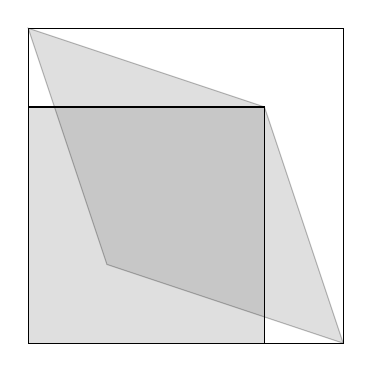
\begin{tikzpicture}
\draw (0,0)--(4,0)--(4,4)--(0,4)--cycle;
\draw[opacity=0.25, fill=black!50!white] (0,0)--(3,0)--(3,3)--(0,3)--cycle;
\draw (0,0)--(3,0)--(3,3)--(0,3)--cycle;
\draw[opacity=0.25, fill=black!50!white] (1,1)--(4,0)--(3,3)--(0,4)--cycle;
\draw (0,0)--(3,0)--(3,3)--(0,3)--cycle;
\end{tikzpicture}

\end{document}